%\documentstyle[epsf,twocolumn]{jarticle}       %LaTeX2e仕様
\documentclass[twocolumn]{jarticle}     %pLaTeX2e仕様(platex.exeの場合)
%\documentclass[twocolumn]{ujarticle}     %pLaTeX2e仕様(uplatex.exeの場合)
%%%%%%%%%%%%%%%%%%%%%%%%%%%%%%%%%%%%%%%%%%%%%%%%%%%%%%%%%%%%%%
%%
%%  基本バージョン
%%
%%%%%%%%%%%%%%%%%%%%%%%%%%%%%%%%%%%%%%%%%%%%%%%%%%%%%%%%%%%%%%%%
\setlength{\topmargin}{-45pt}
%\setlength{\oddsidemargin}{0cm} 
\setlength{\oddsidemargin}{-7.5mm}
%\setlength{\evensidemargin}{0cm} 
\setlength{\textheight}{24.1cm}
%setlength{\textheight}{25cm} 
\setlength{\textwidth}{17.4cm}
%\setlength{\textwidth}{172mm} 
\setlength{\columnsep}{11mm}

\kanjiskip=.07zw plus.5pt minus.5pt


% 【節が変わるごとに (1.1)(1.2) … (2.1)(2.2) と数式番号をつけるとき】
%\makeatletter
%\renewcommand{\theequation}{%
%\thesection.\arabic{equation}} %\@addtoreset{equation}{section}
%\makeatother

%\renewcommand{\arraystretch}{0.95} 行間の設定

%%%%%%%%%%%%%%%%%%%%%%%%%%%%%%%%%%%%%%%%%%%%%%%%%%%%%%%%
\usepackage[dvipdfmx]{graphicx}   %pLaTeX2e仕様(\documentstyle ->\documentclass)\documentclass[dvipdfmx]{graphicx}
\usepackage[dvipdfmx]{color}
\usepackage[subrefformat=parens]{subcaption}
\usepackage{colortbl}
%%%%%%%%%%%%%%%%%%%%%%%%%%%%%%%%%%%%%%%%%%%%%%%%%%%%%%%%

\begin{document}

\twocolumn[
\noindent

\hspace{1em}
\today
\hfill
\ \ 細川 岳大

\vspace{2mm}

\hrule

\begin{center}
{\Large \bf 進捗報告}
\end{center}
\hrule
\vspace{3mm}
]

% ‚ここから 文章 Start!
\section{はじめに}
 近年,機械学習の発展には目を見張るものがあり,画像や自然言語,さらには動画など
 様々なタスクで非常に高い制度を示している.しかし,それらの成果について
 ハイパーパラメータのチューニングやデータ拡張は必須であり,今までは人間が手動で行うことが一般的であった.
 一方で,現在ではそれらについても自動化する研究がなされており,Automated Machine Learning (:AutoML)や
 Auto Augmentと呼ばれている.ところが,これらの探索について
 

\section{実験1}
前回に引き続きGAを用いたアンサンブル学習のためのDataAugmentationの実験を行った.\\

\subsection{実験データ}
実験データはcifar10を用いて,
事前学習ではepoch数300,train\_dataを各ラベル5000枚の計50000枚使用し,GAで学習する際はepoch数100,train\_dataは各ラベル200枚のオリジナルとそれらすべてをDataAugmentaionしたものとを合わせ計4000枚とし,test\_dataは共に10000枚とした.また事前学習でのaccuracyは0.8475である.
\subsection{遺伝的アルゴリズム}


\subsubsection{探索空間}
\ 探索する水増し操作として画素値操作(Sharpness,Posterize,Brightness,Autoconstrast,Equalize,Solarize,Invert,Contrast,ColorBalance),
変形操作(Mirror,Flip,Translate X/Y,Shear X/Y,Rotate)の16種類の操作であり,今回はそれらすべてを個別にどの程度強くかけるかおよびどの順序でかけるかということを探索する.各操作についての強度の最大最小を設定し,それを-100\%から100\%まで25\%ずつ分11段階の度合いとする.ただし,Autocontrast,Equalize,Invert,Mirror については適用するか否かであるためパラメータが0以上で適用するとした.強度は0から5の整数値を持つ15個の遺伝子を実数値コーディングによって表現する.
また,適用順序に関しては同様に15個の遺伝子を持つ順列コーディングによって表現する.
確率は10\%ごと11段階の実数地コーディングによって表現する.
つまり,探索空間は$2^5*11^{11}*15!*11^{16}$となる.

\subsubsection{選択}
\ 選択について,エリート選出によって最も適応度の高い2つの個体を選択する.なお,この二つは後述する交叉,突然変異は受けずに次の世代に追加する.
残りの選出にはトーナメント選出を用した.トーナメント選出は集団の中から任意の数(トーナメントサイズ)の個体のうち最も適応度の高い個体を選出し次の世代に追加する.今回トーナメントサイズは2とした.
 
\subsubsection{交叉}
\ 強度,確率を表す染色体については2点交叉,順序を表す染色体については部分写像交叉を用いた.2点交叉は一対の親染色体をそれぞれ同じ場所で三分割し中央の染色体を入れ替えて交叉を行う.部分写像交叉は親遺伝子を二分割し入れ替える際重複をなくす交叉法で,重複のあった遺伝子について,それに該当した重複する遺伝子座を見つけ,それに対となっているもう一方の親の遺伝子を参照する.
 
\subsubsection{突然変異}
\ 強度,確率を表す染色体について,対象となる遺伝子の値を各50\%の確率に1増減させ,
 順序を表す染色体について,染色体の一部を逆順にする操作か,染色体を二つに分け前後を入れ替える操作のいずれかを行うものとした.
 
\subsubsection{多様性維持}
\ 多様性を維持するために,上記3つの操作(選択,交叉,突然変異)を行った集団に対し,適用順序を表す染色体について一致するものが3つ以上あれば,
それが2つになるように一部の個体を突然変異させたうえで次の世代の集団とした.
 
\subsection{実験1} 
\subsubsection{パラメータ}
表\ref{tb:param1}に学習パラメータを示す.
\begin{table}[h]
	\centering
	\caption{学習パラメータ\label{tb:param1}}
	\scalebox{1.0}{
		\begin{tabular}{|c||c|} \hline
			optimizer&Adam\\ \hline
			learning rate&0.001\\ \hline
			loss function&categorical\_crossentropy\\ \hline
			batch size&128\\ \hline
			epoch size&30\\ \hline
		\end{tabular}
	}
\end{table}
 表\ref{tb:param_GA}にGAの設定を示す.
\begin{table}[h]
	\centering
	\caption{実験パラメータ\label{tb:param_GA}}
	\scalebox{1.0}{
		\begin{tabular}{|c|c|c|} \hline
			\multicolumn{2}{|c|}{個体数}&15\\ \hline
			\multicolumn{2}{|c|}{世代数}&25\\ \hline
			\multicolumn{2}{|c|}{交叉率}&0.9\\ \hline\hline
			\multicolumn{3}{|c|}{突然変異率}\\ \hline
			\multicolumn{2}{|c|}{強度,確率(遺伝子ごと)}&0.06\\ \cline{2-3}
			\multicolumn{2}{|c|}{順序(染色体ごと)}&0.1\\ \hline
		\end{tabular}
	}
\end{table}
\subsubsection{結果}
図\ref{fig:graph1}にaccuracyの最良値及び平均値の推移を示す.
\begin{figure}[hp]
	\centering
	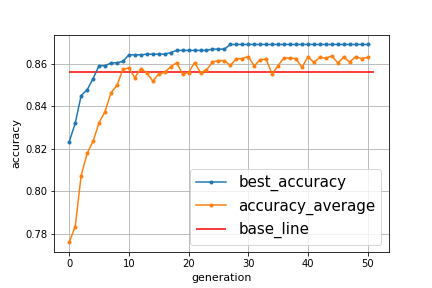
\includegraphics[scale=0.6]{graph.png}
	\caption{accuracyの推移\label{fig:graph1}}
\end{figure}
表\ref{tb:res1}にアンサンブル学習の各世代の最良値を示す.
\begin{table}[h]
	\centering
	\caption{実験結果\label{tb:res1}}
	\scalebox{1.0}{
		\begin{tabular}{|c|c||c|c|} \hline
			1st&0.8576&
			2nd&0.8568\\ \hline
			3rd&0.8581&
			4th&0.8574\\ \hline
			5th&0.8575&
			6th&0.8526\\ \hline
			7th&0.8529&
			8th&0.8534\\ \hline
			9th&0.8521&
			10th&0.8540\\ \hline
			11st&0.8551&
			12nd&0.8566\\ \hline
			13rd&0.8542&
			14th&0.8577\\ \hline
			15th&0.8535&
			\cellcolor[rgb]{0.9,0.9,0}16th&\cellcolor[rgb]{0.9,0.9,0}0.8586\\ \hline
			17th&.8576&
			18th&0.8580\\ \hline
			\cellcolor[rgb]{0.9,0.9,0}19th&\cellcolor[rgb]{0.9,0.9,0}0.8586&
			20th&0.8578\\ \hline
			21th&0.8570&
			22th&0.8573\\ \hline
			23th&.8572&
			24th&0.8575\\ \hline
			25th&0.8578& & \\ \hline
		\end{tabular}
	}
\end{table}
図\ref{fig:graph1}の箱ひげ図よりから程度精度は揃ってきていることが分かる.
一方で各世代のアンサンブル学習についてあまり精度が上がっていない.
また,前回の学習では精度が0.8676となっているので,全体的な精度自体は低い.
記載はしていないが世代を追うごとに,適用順序については制限をかけることでバラバラではあるが,
適用確率,強度は8割程度揃っていた.

\subsection{実験2}
実験1で得られた1,25世代を用いてデータ数を増やして実験を行った

\subsubsection{パラメータ}
表\ref{tb:param2}に学習パラメータを示す.

\begin{table}[h]
	\centering
	\caption{学習パラメータ\label{tb:param2}}
	\scalebox{1.0}{
		\begin{tabular}{|c||c|} \hline
			optimizer&Adam\\ \hline
			learning rate&0.001\\ \hline
			loss function&categorical\_crossentropy\\ \hline
			batch size&128\\ \hline
			epoch&30\\ \hline
		\end{tabular}
	}
\end{table}
元のデータ数は20000とし,DataAugmentationで2倍にして学習を行う.

\subsubsection{結果}
表\ref{tb:res2},表\ref{tb:res3}に結果を示す.

\begin{table}[h]
	\centering
	\caption{1世代\label{tb:res2}}
	\scalebox{1.0}{
		\begin{tabular}{|c|c||c|c|} \hline
			\cellcolor[rgb]{0,0.9,0.9}1st&\cellcolor[rgb]{0,0.9,0.9}0.7943&
			\cellcolor[rgb]{0,0.9,0.9}2nd&\cellcolor[rgb]{0,0.9,0.9}0.8232\\ \hline
			\cellcolor[rgb]{0,0.9,0.9}3rd&\cellcolor[rgb]{0,0.9,0.9}0.7861&
			\cellcolor[rgb]{0,0.9,0.9}4th&\cellcolor[rgb]{0,0.9,0.9}0.4543\\ \hline
			\cellcolor[rgb]{0,0.9,0.9}5th&\cellcolor[rgb]{0,0.9,0.9}0.5574&
			6th&0.6032\\ \hline
			\cellcolor[rgb]{0,0.9,0.9}7th&\cellcolor[rgb]{0,0.9,0.9}0.7725&
			8th&0.7953\\ \hline
			\cellcolor[rgb]{0,0.9,0.9}9th&\cellcolor[rgb]{0,0.9,0.9}0.8042&
			10th&0.7850\\ \hline
			11st&0.7675&
			12nd&0.7498\\ \hline
			\cellcolor[rgb]{0,0.9,0.9}13rd&\cellcolor[rgb]{0,0.9,0.9}0.8101&
			\cellcolor[rgb]{0,0.9,0.9}14th&\cellcolor[rgb]{0,0.9,0.9}0.8182\\ \hline
			\cellcolor[rgb]{0,0.9,0.9}15th&\cellcolor[rgb]{0,0.9,0.9}0.8155& & \\ \hline
			\multicolumn{2}{|c|}{ensemble}&\multicolumn{2}{|c|}{0.8770}\\ \hline
		\end{tabular}
	}
\end{table}

\begin{table}[h]
	\centering
	\caption{25世代\label{tb:res3}}
	\scalebox{1.0}{
		\begin{tabular}{|c|c||c|c|} \hline
			1st&0.8162&
			\cellcolor[rgb]{0,0.9,0.9}2nd&\cellcolor[rgb]{0,0.9,0.9}0.8434\\ \hline
			3rd&0.8373&
			\cellcolor[rgb]{0,0.9,0.9}4th&\cellcolor[rgb]{0,0.9,0.9}0.8343\\ \hline
			5th&0.8377&
			\cellcolor[rgb]{0,0.9,0.9}6th&\cellcolor[rgb]{0,0.9,0.9}0.8096\\ \hline
			\cellcolor[rgb]{0,0.9,0.9}7th&\cellcolor[rgb]{0,0.9,0.9}0.8359&
			8th&0.8385\\ \hline
			\cellcolor[rgb]{0,0.9,0.9}9th&\cellcolor[rgb]{0,0.9,0.9}0.8243&
			\cellcolor[rgb]{0,0.9,0.9}10th&\cellcolor[rgb]{0,0.9,0.9}0.8388\\ \hline
			\cellcolor[rgb]{0,0.9,0.9}11st&\cellcolor[rgb]{0,0.9,0.9}0.8289&
			\cellcolor[rgb]{0,0.9,0.9}12nd&\cellcolor[rgb]{0,0.9,0.9}0.8394\\ \hline
			\cellcolor[rgb]{0,0.9,0.9}13rd&\cellcolor[rgb]{0,0.9,0.9}0.8346&
			\cellcolor[rgb]{0,0.9,0.9}14th&\cellcolor[rgb]{0,0.9,0.9}0.8165\\ \hline
			15th&0.8388& & \\ \hline
			\multicolumn{2}{|c|}{ensemble}&\multicolumn{2}{|c|}{0.8732}\\ \hline
		\end{tabular}
	}
\end{table}

アンサンブル学習について25世代の個体を使うよりも,1世代の個体を使う方が精度が高くなった.


\subsection{考察}
\ 今回の実験では,適用順序の染色体の重複数を制限することで順序の多様性は確保できた一方で,
適用確率や強度についてはの多様性は保たれていない.そのため順序が逆でも同等になる変換がある可能性から,
個体同士自体の多様性は低い可能性がある.
そのため,実験2では多様性の高い1世代目のほうがアンサンブル学習がうまくいったのではないかと考えられる.
\ 表\ref{tb:res2}のようにアンサンブル学習について個々の精度が高いほど良いのかもしれないが,
より時に精度が低いものも混ぜる必要があると考えられる.そのため今回の実験において適応度は各個別の精度であり,
次の世代に持ち越すのにアンサンブル学習について全く考慮していないものとなっていたので,
個々の精度に加えてアンサンブル学習において良い精度を出した時に選出された個体に対しある程度の重みを付加する必要が
あると思う.

\section{今後の課題}
\begin{itemize}
	\item 適応度の計算についてアンサンブル学習での結果を考慮したものを試してみる
\end{itemize}

\end{document}


